\chapter{Conclusioni}
\label{cap:conclusioni}


\section{Raggiungimento degli obiettivi}
Per terminare il percorso di stage è necessario verificare il grado di soddisfacimento degli obiettivi preimposti, tale processo viene rappresentato nella tabella \ref{soddisfazione}.
L'implementazione del sistema di cattura rispecchia completamente le aspettative e funziona in maniera corretta, integrandosi inoltre con il database preesistente.
I requisiti desiderabili e facoltativi, come l'inserimento e l'aggiornamento della valutazione dei siti web, sono risultati una naturale estensione del processo di valutazione tramite IA e quindi sono stati implementati come se facessero parte del medesimo obiettivo.
L'automazione dell'invio delle e-mail è stata preparata e testata, ma per motivi di sicurezza necessita ancora dell'approvazione di un supervisore prima di lanciare la campagna di invio.
Nelle sotto sezioni successive è presente un'analisi più dettagliata dei processi fondamentali del processo.

\newpage
\begin{table}[!htbp]
    \centering
    \begin{tabularx}{0.8\textwidth}{|c|X|X|}
    \hline
    \textbf{Codice} & \textbf{Descrizione} & \textbf{Soddisfacimento}\\
    \hline
    O01 & Implementare un sistema robusto per la cattura degli screenshot, assicurando l’integrazione con il database per l’archiviazione e l’analisi. & Soddisfatto\\
    \hline
    O02 & Garantire la creazione di una documentazione tecnica completa che supporti sia l’uso che la manutenzione  del sistema sviluppato. & Soddisfatto\\
    \hline
    O03 & Creazione di un IA in grado di suddividere in cluster i siti web. & Soddisfatto\\
    \hline
    O04 & Creazione di un IA classificativa in grado di assegnare un punteggio ai siti web analizzati. & Soddisfatto\\
    \hline
    D01 & Aggiungere la valutazione creata dall'IA nel database utilizzato dal CRM. & Soddisfatto\\
    \hline
    D02 & Automatizzare l'invio di e-mail alle aziende che hanno ottenuto una valutazione scarsa. & Soddisfatto\\
    \hline
    F01 & Migliorare la raccolta dei dati delle aziende dal web & Non soddisfatto\\
    \hline
    F02 & Aggiornare automaticamente la valutazione dei siti web & Soddisfatto\\
    \hline
    \end{tabularx}
    \caption{Grado di soddisfacimento degli obiettivi}
    \label{soddisfazione}
\end{table}


\newpage 

\subsection{Clustering}
I risultati di \emph{clustering} migliori sono stati ottenuti con l'estrazione delle \emph{feature} tramite ResNet50, ma il processo necessita di ulteriori ottimizzazioni per essere funzionale;
infatti visualizzando manualmente i cluster ottenuti non è possibile notare delle distinzioni nette tra immagini appartenenti a una o all'altra categoria. Ciò potrebbe essere imputabile alla natura del \emph{dataset}, le immagini di siti web non sono dei soggetti semplici da analizzare, poiché ricche di informazioni come immagini relative al contesto, che non sono utili per giudicare la qualità.
Ad esempio prendiamo in considerazione il sito web dell'università e il sito di un centro estetico che offre servizi di manicure (Fig.~\ref{fig:unipd-conc}).
Le due immagini contengono rappresentazioni di mani, di conseguenza potrebbero essere inserite all'interno dello stesso cluster nonostante facciano parte di contesti diametralmente opposti.
\begin{figure}[!h] 
    \centering 
    
\includegraphics[width=0.8\columnwidth]{conclusioni/unipd.png} 
    \caption{Immagini appartenenti a contesti differenti}
    \label{fig:unipd-conc}
  \end{figure}

\newpage
Un'altra combinazione è dettata da appartenenza alla medesima categoria e differenza di qualità (Fig.~\ref{fig:computer-conc}).
In questo caso la presenza dei computer potrebbe comportare l'inserimento nello stesso cluster, ma come è possibile notare, ciò non sarebbe utile ai fini del progetto, perché si unirebbe un sito web di buona qualità a uno che utilizza tecnologie molto arretrate.

\begin{figure}[!h] 
    \centering 
    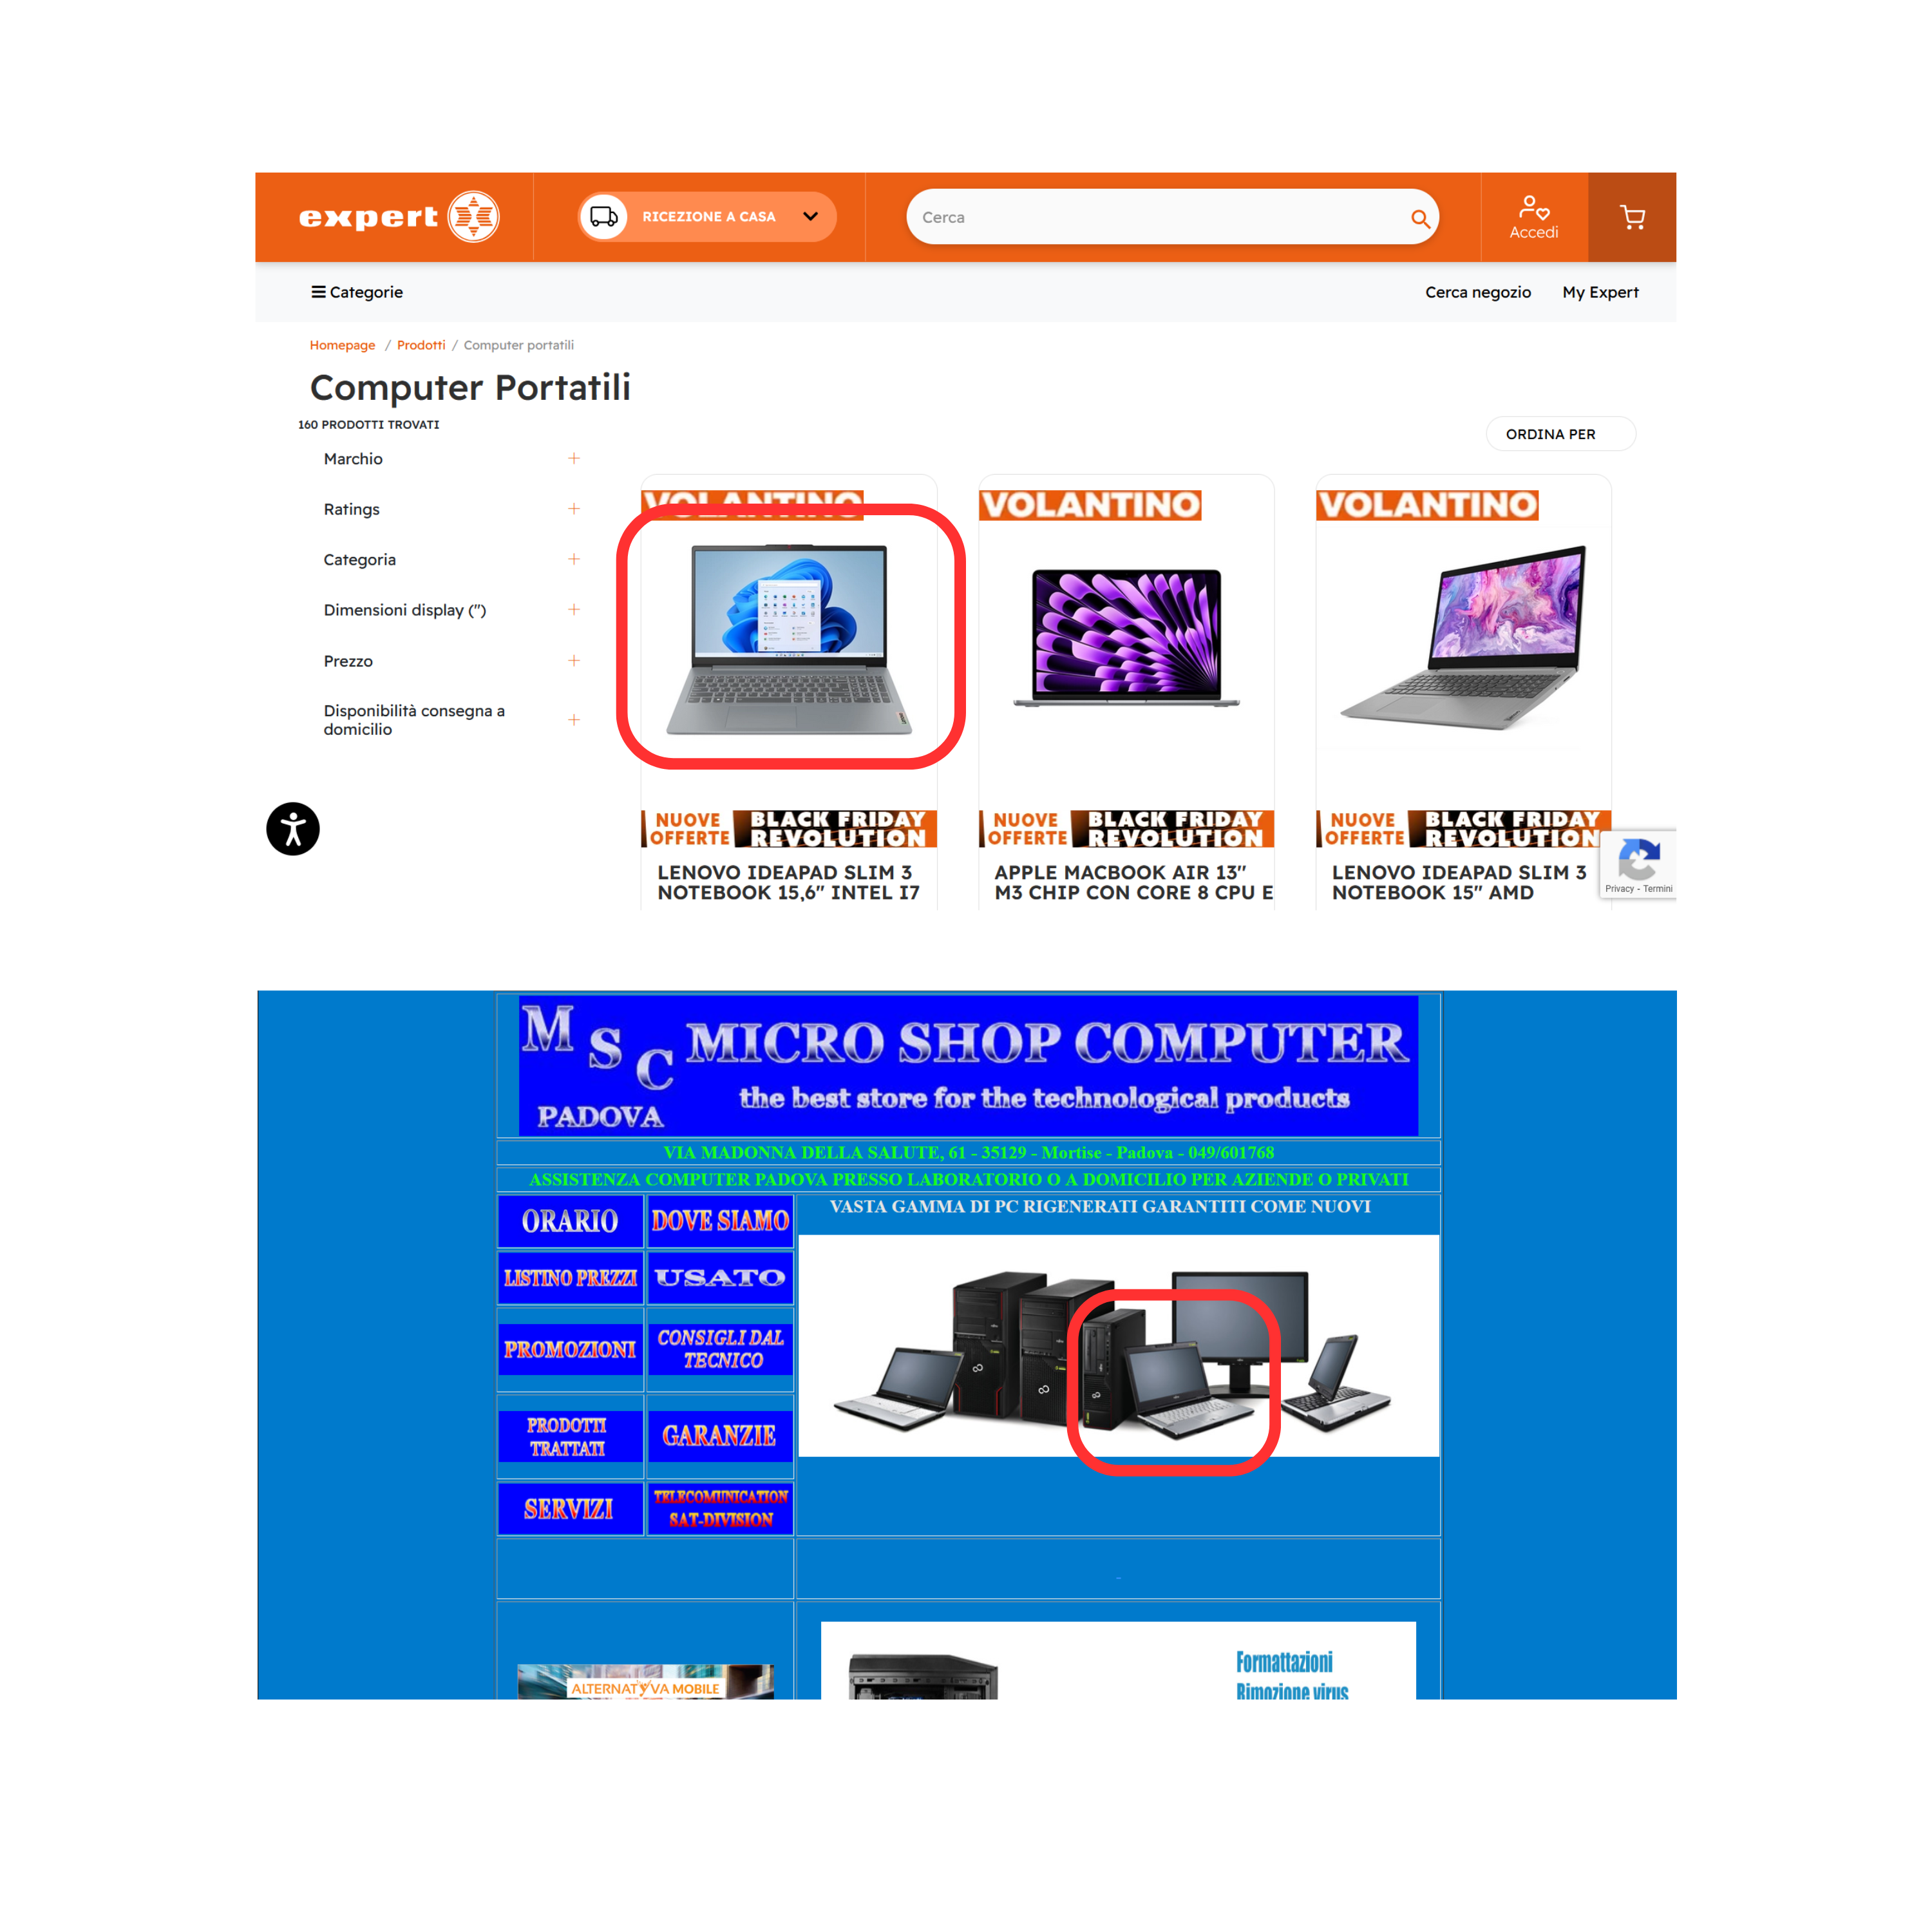
\includegraphics[width=0.8\columnwidth]{conclusioni/computer.png} 
    \caption{Immagini appartenenti allo stesso contesto}
    \label{fig:computer-conc}
  \end{figure}

Per migliorare il \emph{clustering} ci si potrebbe concentrare solo su parti specifiche del sito web rendendo l'analisi più indipendente da informazioni non utili; inoltre si potrebbe rivalutare l'utilizzo della PCA, effettuando uno studio sulla dimensionalità ottimale dello spazio delle \emph{feature}. (Tale scelta comporta un probabile miglioramento dei risultati ma compromette la facile interpretabilità dei grafici).
Per procedere con il progetto risulta anche necessario comprendere più a fondo come utilizzare l'algoritmo K-means al meglio e testare altri algoritmi di \emph{clustering}.
Il lavoro svolto può essere considerato un'ottima base di partenza poiché si è concentrato sullo studio preliminare di varie metodologie; arrivando a escludere quelle meno adatte al compito di estrazione delle \emph{feature}.

\subsection{Valutazione delle immagini}
Per quanto riguarda la fase di valutazione, i risultati ottenuti dal \emph{fine tuning} di ResNet50 sembrano essere ottimali, ottenendo un'accuratezza del 92\%.
La rete neurale è inoltre risultata capace di assegnare valutazioni congrue a quelle che lo sviluppatore si aspetterebbe di visualizzare; ossia voti che vanno da 0 a 100 in un range che spazia da siti molto antiquati e nettamente migliorabili a siti ottimi che non necessitano modifiche.
Il prodotto è comunque migliorabile aggiungendo una quantità più elevata di screenshot al \emph{dataset} e di conseguenza aumentando il range di siti a cui adattarsi.

\section{Valutazione personale}
L'esperienza di stage è stata di grande impatto, ha consentito di sfruttare le conoscenze acquisite e ha messo in risalto numerose lacune da colmare.
Il progetto mi ha consentito di apprendere nuove conoscenze nell'ambito del \emph{machine learning}, argomento che personalmente non avevo mai approfondito. 
Le scarse conoscenze in ambito IA hanno comportato una grossa sfida, che una volta superata ha portato a un alto livello di soddisfazione.

